\documentclass[journal,12pt,twocolumn]{IEEEtran}
\usepackage{tikz}
\usepackage{amsmath}
\usepackage{breqn}
\usepackage{amssymb}
\pagestyle{empty}
\usepackage{setspace}
\usepackage{gensymb}
\singlespacing

\usepackage{amsmath}
\usepackage{amsthm}
\begin{document}
\providecommand{\sbrak}[1]{\ensuremath{{}\left[#1\right]}}
\providecommand{\lsbrak}[1]{\ensuremath{{}\left[#1\right.}}
\providecommand{\rsbrak}[1]{\ensuremath{{}\left.#1\right]}}
\providecommand{\brak}[1]{\ensuremath{\left(#1\right)}}
\providecommand{\lbrak}[1]{\ensuremath{\left(#1\right.}}
\providecommand{\rbrak}[1]{\ensuremath{\left.#1\right)}}
\providecommand{\cbrak}[1]{\ensuremath{\left\{#1\right\}}}
\providecommand{\lcbrak}[1]{\ensuremath{\left\{#1\right.}}
\providecommand{\rcbrak}[1]{\ensuremath{\left.#1\right\}}}
\let\StandardTheFigure\thefigure
\let\vec\mathbf

\title{
Assignment - 1
}
\author{ Soham Bhatt \\SM21MTECH14004}
\maketitle
\newpage
\bigskip
\bibliographystyle{IEEEtran}
\section*{\textbf{Problem}}
\noindent
\textbf{\textsl{1. Show that the diameter of the circum-circle formed by the points A(r,$\theta$), B($\rho$,$\theta$) and the pole is:
$$ \frac{\sqrt{{r}^2+{\rho}^2-2r\rho\cos{(\theta-\phi)}}}{\sin{(\phi-\theta)}} $$ }}

\noindent
\section*{\textbf{Solution}}
\noindent

$$$$
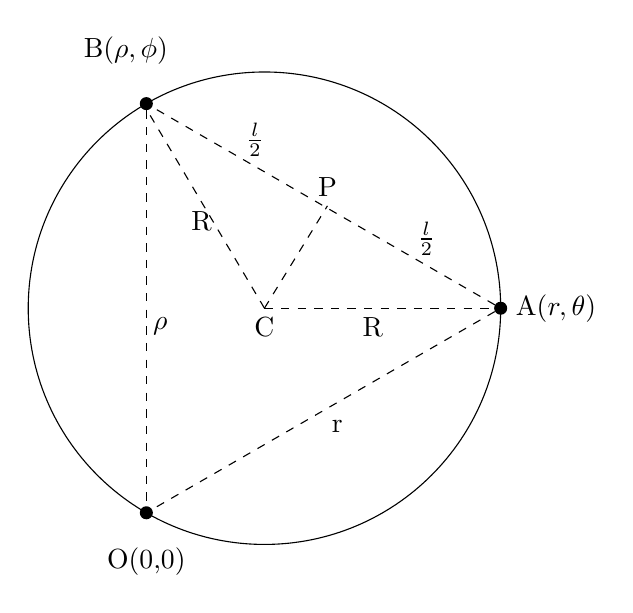
\begin{tikzpicture}

    % equidistant points and arc
    \foreach \x [count=\p] in {0,...,2} {
        \node[shape=circle,fill=black, scale=0.5] (\p) at (-\x*120:3) {};};
    \foreach \x [count=\p] in {0,1,2} {
        \draw (-\x*120:3.6);}
        /%\draw (-30-\x*60:3.6) node {$\bar{\p}$};}; 
    \draw (1) arc (0:360:3);
    \draw[dashed] (1) -- (2) node[pos=0.5, below]{\quad r};
    \draw[dashed] (3) -- (2) node[pos=1.2, above]{O(0,0)} node[pos=0.5, below]{\quad$\rho$};
    \draw[dashed] (1) -- (3) node[pos=0.7, above] {$\frac{l}{2}$} node[pos=0.2, above] {$\frac{l}{2}$};;
    % axes
    \draw [dashed] (0,0) -- (3,0)  node{\qquad\quad\quad A$(r,\theta)$} node[pos=0.4, below]{\quad R};
    \draw [dashed] (0,0) -- (-1.6,2.7) node[pos=1.1, above]{B$(\rho,\phi)$} node[pos=0.5, below]{R};
    \draw [dashed] (0,0) -- (0.8,1.3) node[pos=1, above]{P} node[pos=0, below]{C};
    
\end{tikzpicture}
$$$$

We know that area of $\Delta OAB $ with vertices $(0,0)$, $(\theta, \phi)$, $(r,\phi)$ is given by
$$ A_t = \frac{1}{2}(OA)(OB)(\sin(\phi-\theta)) $$
$$ A_t = \frac{1}{2}r\rho\sin(\phi-\theta) \qquad (1)$$ 

Now, by right angle triangle $\Delta PCB $,
$$ \sin(\phi-\theta) = \frac{\frac{l}{2}}{R} = \frac{l}{2R} \qquad (2) $$
$$(where R is radius of the circle)$$

Substituting values of (2) in (1), we get
$$ A_t = \frac{1}{2}r\rho(\frac{l}{2R}) $$
$$ \frac{1}{2}r\rho\sin(\phi - \theta) = \frac{1}{2}r\rho(\frac{l}{2R}) $$
$$ \sin(\phi-\theta) = \frac{l}{2R} $$
$$ R = \frac{l}{2\sin(\phi-\theta)} = Radius\quad of\quad circum\quad circle $$
$$  D = 2R = \frac{l}{\sin(\phi-\theta)} \qquad(3) $$
$$ (Where D is Diameter of circum circle) $$

But we know that, the distance between two points $A(r,\theta)$ and $B(\rho,\phi)$ is,
$$ AB = l = \sqrt{r^2 + \rho^2 - 2r\rho\cos(\theta-\phi)} $$
From (3),
$$ D = \frac{\sqrt{r^2 + \rho^2 - 2r\rho\cos(\theta-\phi)}}{\sin(\phi - \theta)} $$

\end{document}